\documentclass[solution,addpoints,12pt]{exam}
\printanswers
\usepackage{amsmath,amssymb}
\usepackage{multirow}
\usepackage{enumitem}
\usepackage[colorlinks=true, linkcolor=blue, urlcolor=blue]{hyperref}
\newcommand{\RP}{\ensuremath{\mathsf{RP}}}
\newcommand{\expect}[1]{\ensuremath{\mathbb{E}[#1]}}
\newcommand{\dx}{\mathrm{d}x}
\usepackage{graphicx}
\pointpoints{mark}{marks}

\begin{document}

\hrule
\vspace{1mm}
\noindent 
\begin{center}
{\Large CS6700 : Reinforcement Learning} \\
{\large Written Assignment \#3}
\end{center}
%\hfill Release date: 21 Jan, 2017, 12:00 pm}
\vspace{1mm}
\noindent 
{\large \hfill Deadline: ??}

\vspace{2mm}
\hrule

{\small

\begin{itemize}\itemsep0mm
\item This is an individual assignment. Collaborations and discussions are strictly
prohibited.
\item Be precise with your explanations. Unnecessary verbosity will be penalized.
\item Check the Moodle discussion forums regularly for updates regarding the assignment.
\item \textbf{Please start early.}
%\item Turn in \textbf{only the answers} on Turnitin.
\end{itemize}
}

\hrule

\vspace{3mm}
\noindent {\sc Author :} Name. \\[1mm]
\noindent {\sc Roll Number :} \\
%\hrule


\begin{questions}
\question[3] Consider the problem of solving POMDPs using Deep Reinforcement Learning. Can you think of ways to modify the standard DQN architecture to ensure it can remember histories of states. Does the experience replay also need to be modified? Explain.

\begin{solution}

\end{solution}


\question[4] Exploration is often ameliorated by the use of counts over the various states. For example, one could maintain a visitation count $N(s)$, for every state and use the same to generate an intrinsic reward ($r_i(s)$) for visiting that state.
\[ r_i(s) = \tau \times \frac{1}{N(s)} \]
However, it is intractable to maintain these counts in high-dimensional spaces, since the count values will be zero for a large fraction of the states. Can you suggest a solution(s) to handle this scenario? How can you maintain an approximation of the counts for a large number of states and possibly generalize to unseen states?

\begin{solution}

\end{solution}

\question[5] Suppose that the MDP defined on the observation space is k-th order Markov, i.e. remembering the last k observations is enough to predict the future. 
Consider using a belief state based approach for solving this problem. For any starting state and initial belief, the belief distribution will localize to the right state after k updates, i.e., the true state the agent is in will have a probability of 1 and the other states will have a probability of 0. Is this statement true or false? Explain your answer. 

\begin{solution}

\end{solution}




\question[3]
Q-MDPs are a technique for solving the problem of behaving in POMDPs. The behavior produced by this approximation would not be optimal. In what sense is it not optimal?  Are there circumstances under which it can be optimal?

\begin{solution}

\end{solution}

\question[3] What are some advantages and disadvantages of A3C over DQN? What are some potential issues that can be caused by asynchronous updates in A3C?

\begin{solution}

\end{solution}

\question[6] There are a variety of very efficient heuristics available for solving deterministic travelling salesman problems. We would like to take advantage of such heuristics in solving
certain classes of large scale navigational problems in stochastic domains. These problems involve navigating from one well demarcated region to another. For e.g., consider
the problem of delivering mail to the office rooms in a multi storey building.

\begin{parts}
    \part[4] Outline a method to achieve this, using concepts from hierarchical RL.
    \begin{solution}
    
    \end{solution}
    \part[2] What problems would such an approach encounter?
    \begin{solution}
    
    \end{solution}
\end{parts}

\question[6] This question may require you to refer to \href{this}{https://link.springer.com/content/pdf/10.1007/BF00114727.pdf} paper on average reward RL. Consider the 3 state MDP shown in Figure \ref{fig:avg}.  Mention the recurrent class for each such policies. In the average reward setting, what are the corresponding $\rho^{\pi}$ for each such policy ? Furthermore, which of these policies are gain optimal ? 
    \begin{parts}
        \part[3] What are the different deterministic uni-chain policies present ?
        \part[3] In the average reward setting, what are the corresponding $\rho^{\pi}$ for each such policy ? Furthermore, which of these policies are gain optimal ? 
    \end{parts}

    \begin{figure}[h]
        \centering
        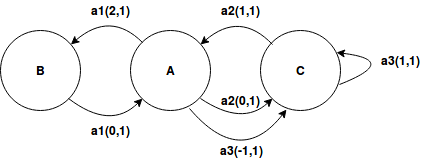
\includegraphics[scale=0.6]{average_reward.png}
        \caption{Notation : action(reward, transition probability). Example : a1(3, 1) refers to action a1 which results in a transition with reward +3 and probability 1}
        \label{fig:avg}
    \end{figure}

\end{questions}


\end{document}